\documentclass[onecolumn, draftclsnofoot,10pt, compsoc]{IEEEtran}
\usepackage{graphicx}
\usepackage{url}
\usepackage{setspace}
\usepackage[font=small,labelfont=bf]{caption} % Required for specifying captions to tables and figures
\usepackage{geometry}
\geometry{textheight=9.5in, textwidth=7in}

% 1. Fill in these details
\def \CapstoneTeamName{		Malsano}
\def \CapstoneTeamNumber{		72}
\def \GroupMemberOne{			Katherine Jeffrey}
\def \GroupMemberTwo{			Brandon Jolly}
\def \GroupMemberThree{			Bradford Wong}
\def \CapstoneProjectName{		App to Support Field Diagnostics in Veterinary Medicine}
\def \CapstoneSponsorCompany{	Oregon Veterinary Diagnostics Laboratory}
\def \CapstoneSponsorPerson{		Professor Christiane Loehr}

% 2. Uncomment the appropriate line below so that the document type works
\def \DocType{		%Problem Statement
				%Requirements Document
				%Technology Review
				Design Document
				%Progress Report
				}

\newcommand{\NameSigPair}[1]{\par
\makebox[2.75in][r]{#1} \hfil 	\makebox[3.25in]{\makebox[2.25in]{\hrulefill} \hfill		\makebox[.75in]{\hrulefill}}
\par\vspace{-12pt} \textit{\tiny\noindent
\makebox[2.75in]{} \hfil		\makebox[3.25in]{\makebox[2.25in][r]{Signature} \hfill	\makebox[.75in][r]{Date}}}}
% 3. If the document is not to be signed, uncomment the RENEWcommand below
%\renewcommand{\NameSigPair}[1]{#1}

%%%%%%%%%%%%%%%%%%%%%%%%%%%%%%%%%%%%%%%
\begin{document}
\begin{titlepage}
    \pagenumbering{gobble}
    \begin{singlespace}
    	%
\includegraphics[scale=1, bb=0 0 30 30]{coe_v_spot1.eps}
        \hfill
        % 4. If you have a logo, use this includegraphics command to put it on the coversheet.
        %\includegraphics[scale=1, bb=0 0 30 30]{CompanyLogo}
        \par\vspace{.2in}
        \centering
        \scshape{
            \huge CS Capstone \DocType \par
            {\large\today}\par
            \vspace{.5in}
            \textbf{\Huge\CapstoneProjectName}\par
            \vfill
            {\large Prepared for}\par
            \Huge \CapstoneSponsorCompany\par
            \vspace{5pt}
            {\Large\NameSigPair{\CapstoneSponsorPerson}\par}
            {\large Prepared by }\par
            Group\CapstoneTeamNumber\par
            % 5. comment out the line below this one if you do not wish to name your team
            \CapstoneTeamName\par
            \vspace{5pt}
            {\Large
                \NameSigPair{\GroupMemberOne}\par
                \NameSigPair{\GroupMemberTwo}\par
                \NameSigPair{\GroupMemberThree}\par
            }
            \vspace{20pt}
        }
        \begin{abstract}
        % 6. Fill in your abstract
        	Currently, there are many difficulties for veterinary pathologists trying to perform remote diagnostics. There are not any effective ways for people out in the field collecting samples to communicate with specialized experts located in laboratories. As a result, this project will involve creating an android mobile application that will be used as a bridge to connect the field personnel with the veterinary pathologists in laboratories. With this mobile application, the field personnel will be able to take pictures of the individual that is being analyzed and then send the pictures along with other data such as the patient, location, and time to a pathologist. The pathologist will then be able to use the provided information to perform a necropsy and send feedback to the field personnel. This project is intended to support remote field diagnostics in veterinary medicine.
        \end{abstract}
    \end{singlespace}
\end{titlepage}
\newpage
\pagenumbering{arabic}
\tableofcontents
% 7. uncomment this (if applicable). Consider adding a page break.
%\listoffigures
%\listoftables
\clearpage

% 8. now you write!
\section{Introduction}
The completed project components are intended to serve as a means of communication between personnel in the field and pathologists in the laboratory. It's purpose is to improve a team's ability to perform remote diagnostics by providing a convenient way for teams to communicate information. The OVDL wants a native Android mobile application that collects field data and images, stores the information on a native SQLite database, sends them to the lab's MySQL database, and gets real time feedback from the lab. The lab will interact with the database and user's submissions through the website.

%Bradford's Components
\section{Android Application}
\subsection{Home Screen}
There will be four NavButtons (described later). Clicking on each button will take the user to the corresponding page. The NavButtons will be contained in a vertical linear layout. Here is a list of each button and what their attributes will be:
\begin{itemize}
\item A button with an image of a person’s shape for the image, light green for the background color, and “"Create Account"” for the text. Clicking on this button will open up the web browser and take the user to the registration page
\item A button with a plus icon for the image, blue for the background color, and "“Create submission”" for the text
\item A button with a closed folder icon for the image, red for the background color, and “"View submission"” for the text
\item A button with an icon an open folder for the image, dark green for the background color, and “"View Drafts”" for the text
\end{itemize}

\begin{center}
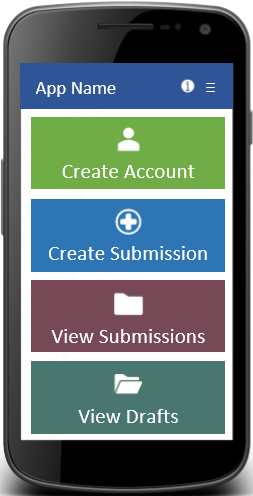
\includegraphics[height=8cm]{homescreen.png}
\end{center}
\captionof{figure}{Home Screen Mockup}


\subsection{NavButton}
This custom class will inherit from the Button class. It's attributes should include an image, background color, and text. All the text color will be set by default to white. The class should also have getter and setter functions for each of the attributes.

\subsection{Toolbar Menu}
This will use the Toolbar class. Every page will have a toolbar, and the text in the toolbar will be the same as the current screen's name. There will be an overflow menu on the right of the toolbar with the following options: "Home", "Create submission", "View Submissions", "Instructions", and "Settings". Clicking on one option will take the user to the corresponding page.
\newline
\begin{center}
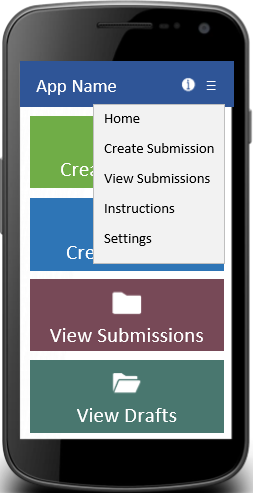
\includegraphics[height=8cm]{menuscreen.png}
\end{center}
\captionof{figure}{Menu Screen Mockup}


\subsection{Create Submission Screen}
There will be a combination of text fields and dropdown menus. The Spinner class will be used for the drop down menus and the EditText class will be used for text fields. There will be a button that says "Submit". Clicking on this button will create a submission in the phone's database and save all the submitted information. It will then try to send the submission to the database if there is an internet connection. There will also be a button that says "Save Draft", which will store the current draft with all its filled out information on the phone's database. There will also be a button with a camera icon on it. Clicking on it will take the user to the page where they can add and remove pictures to the submission. The icon will also have a badge, which will say the number of pictures that were added to the submission.
\newline
\begin{center}
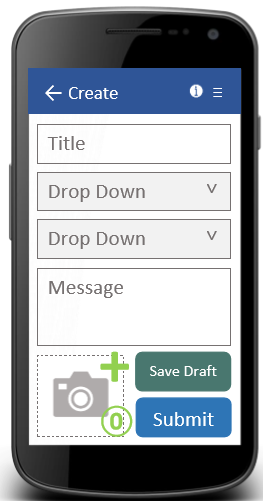
\includegraphics[height=8cm]{createscreen.png}
\end{center}
\captionof{figure}{Create Screen Mockup}

\subsection{Adding Pictures Screen}
This screen will use a grid layout. Each element will be of the ImageButton class. If a picture hasn't been added to a cell, then the cell's image will be a camera icon. If a picture has already been added, then the image will be the actual picture that was added. There will also be a floating, circular button on the bottom right of the screen with a checkmark icon. It will be of the FloatingActionButton class. Clicking on it will save the images and return the user back to the "Create" screen. The grid will have the following properties:
\newline
\begin{center}
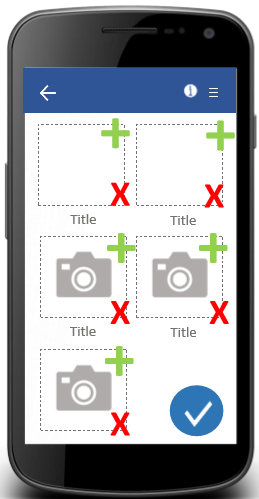
\includegraphics[height=8cm]{picturesscreen.png}
\end{center}
\captionof{figure}{Picture Screen Mockup}

\begin{itemize}
\item The grid will have two total columns
\item The first column will have three elements
\item The second column will have two elements
\end{itemize}

\subsection{Past Submissions Screen}
This screen will have a ListView with a Custom Adapter in order to populate the rows. Each row will have the title of the submission and the date it was created. Each row will also have the Case ID in green text if it was successfully sent to the server. If it wasn't sent successfully or is waitint for an internet connection, then it will be red. Clicking on an entry will navigate the user to the detailed page of that submission.

\subsection{View Submissions Screen}
This screen will have a vertical LinearLayout where all of the information in the submission is added to the layout. The pictures of the submission will show up in a GridLayout. The pictures will initially just have a camera icon. Clicking on the icon will actually download the image.
\newline
\begin{center}
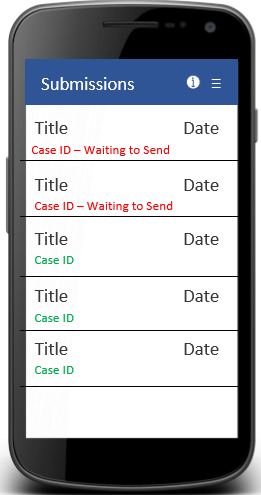
\includegraphics[height=8cm]{submissionscreen.png}
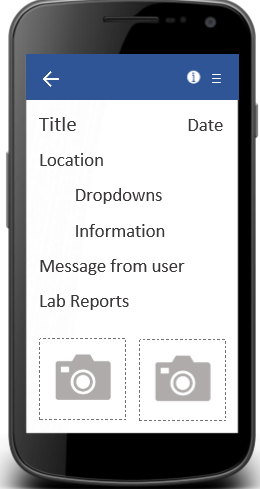
\includegraphics[height=8cm]{detailsscreen.png}
\end{center}
\captionof{figure}{Submissions and Details Screen Mockups}

%Katherine's Components
\subsection{Settings Screen}
The settings screen will have a logout button that will remove the users account credentials from the phone’s local storage. They will need to authenticate their account again before they can save or send a submission. There will be a login button that will prompt the user with a customized AlertDialog for their username and password to save their credentials to the phone’s local storage. To do this they must have an internet connection so their credentials can be matched in the database.
\begin{center}
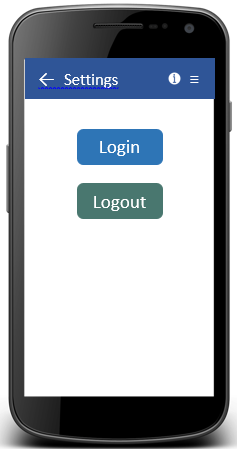
\includegraphics[height=8cm]{settingsscreen.png}
\end{center}
\captionof{figure}{Settings Screen Mockup}

\subsection{Instructions Screen}
The instructions screen will have lists of steps explaining how to use the app, how to register an account, how to create a submission, and how to send messages attached to the submissions. There will also be a link to the website and contact information for the OVDL.
\newline
\begin{center}
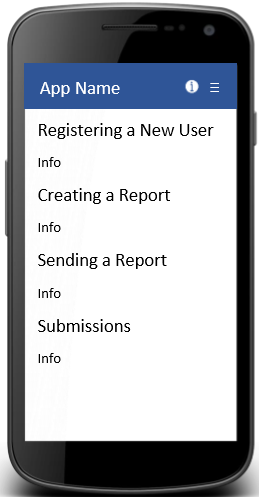
\includegraphics[height=8cm]{instructionsscreen.png}
\end{center}
\captionof{figure}{Instructions Screen Mockup}


%Brandon's Components
\section{Database}
\subsection{Overview}
This project will utilize two databases using the structure presented in the figure below. One database is a MySQL database which will be storing the majority of the information for the app. This will be stored on an apache server and the information will be accessed using a web interface. Our second database is SQLite. The reason for this second database is to allow field workers to store information on the app while not connected to the internet. Instead the database will be stored locally within the phone and will only contain the current user's information.

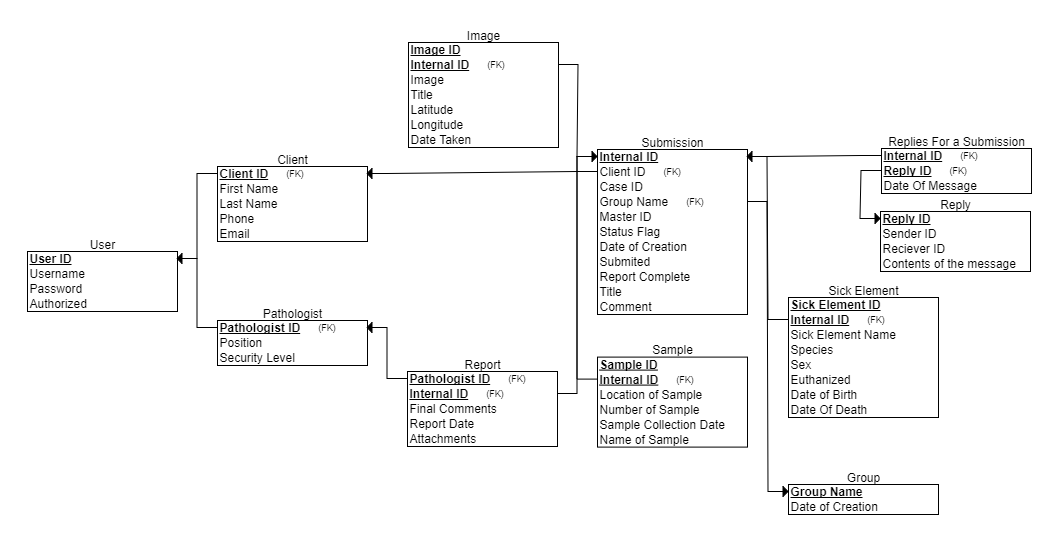
\includegraphics[height = 8cm]{ER_diagram.png}
\captionof{figure}{ER Diagram}

\subsection{Data Dictionary}
\begin{itemize}
\item User:\newline
A parent table to the Client, and Pathologist tables. Will contain the username, password, and if the user has advanced permissions.
\begin{itemize}
\item User ID: The primary key which is a unique integer value generated using a running total. Created when a new user is added to the table.
\item Username: A unique varchar(16) value created when a user creates an account using the web interface.
\item Password: A varchar(16) value created when a user creates an account using the web interface.
\item Authorized: A binary value representing if a user has permission to modify reports, delete reports, etc.
\end{itemize}

\item Client:\newline
A child of the User table. In addition to the information provided by the User table the Client table also contains the contact information. Clients are users who create submissions for a Pathologist to report.
\begin{itemize}
\item Client ID: A foreign key from the User table and the Primary key for the Client table.
\item First Name: A varchar(30) value containing the user's first name.
\item Last Name: A varchar(30) value containing the user's last name.
\item Phone Number: A varchar(16) value containing the user's phone number in "XXX-XXX-XXXX" format.
\item Email: A varchar(40) value containing the user's email address.
\end{itemize}

\item Pathologist:\newline
A child of the User table. In addition to the information provided by the User table the Pathologist table will also contain the position of the pathologist, and what security level the have. Pathologists are the ones who will be reviewing the submissions using reports.
\begin{itemize}
\item Pathologist ID: A foreign key from the User table, and the Primary key for the Pathologist table.
\item Position: A varchar(60) value containing what position a Pathologist holds. (Assistant, Director, etc.)
\item Security Level: An interger value used to determine what permissions a pathologist is able to use.
\end{itemize}

\item Submission:\newline
The submission table contains submissions a Client creates and then sends to a Pathologist to review.
\begin{itemize}
\item Internal ID: The primary key for the Submission table. It is created using a running total on the SQLite database.
\item Client ID: A foreign key from the Client table to determining which client has created the report.
\item Case ID: An integer number created by using the last two digits of the year and then a six digit running total. It's primary use is to allow a pathologist to easily recognizing what submission they are working on. May be dropped in the future when the Use of this app expands.
\item Sick Element ID: A foreign key from the Sick Element table to determine what animal the submission is currently based on.
\item Group Name: A foreign key from the Group table which holds what group this submission is apart of. Defaulted to blank.
\item Master ID: An integer which is filled when the submission is sent to the MySQL database. This will become the primary key in the MySQL But will be a searchable value in the SQLite database.
\item Date of Creation: A datetime value representing the date the submission was first created. Formated as "YYYY/MM/DD HH:MM".
\item Submitted: A datetime value representing when the submission was sent to the MySQL database. Formated as "YYYY/MM/DD HH:MM".
\item Report Complete: A datetime value for when the submission has been closed and the reports for the submission have been finished. Formated as "YYYY/MM/DD HH:MM".
\item Title: A varchar(255) value containing the title a Client Created. The title has to be unique for the client only.
\item Comment: A varchar(255) value containing the comments a Client inputed when they where creating the submission.
\end{itemize}

\item Image:\newline
The Image table contains the images used in a submission. There could be many images which belong to the same submission. Also contains where the image was taken, when it was taken, and a Client created title.
\begin{itemize}
\item Image ID: The primary key for the image table. Created using a running total for the specific submission.
\item Internal ID: A foreign key from the Submission table and a primary key in combination with Image ID.
\item Image: A varchar(255) containing the image file.
\item Title: A varchar(255) containing a user created title. Only has to be unique to the submission.
\item Latitude: A floating point value containing the latitude coordinates.
\item Longitude: A floating ponit value containing the longitude coordinates.
\item Date Taken: A datetime value containing when the picture was taken. Formated as "YYYY/MM/DD HH:MM".
\end{itemize}

\item Sick Element:\newline
The Sick Element table contains the information regarding the animal in a submission. Such as the animal's name, it's sex, etc.
\begin{itemize}
\item Sick Element ID: A primary key, an integer value which is generated with a running total on the SQLite database.
\item Internal ID: A foreign key from the submission table. A primary key in combination with the Sick Element ID.
\item Sick Element Name: A varchar(30) value contain a Client created name for the animal.
\item Species: A varchar(30) value containing what species the animal is.
\item Sex: A varchar(1) value containing the sex of the animal. M for male, and F, for female.
\item Euthanized: A binary value representing if the animal is euthanized or not.
\item Date of Birth: A date value representing the birthday of the animal. Formated as "YYYY/MM/DD".
\item Date of Death: A date value representing the date of death for the animal. Formated as "YYYY/MM/DD".
\end{itemize}

\item Sample:\newline
The Sample table contains the information associated with the sample of the submission.
\begin{itemize}
\item Sample ID: A primary key in the form of an integer value. Generated with a running total on the SQLite Database.
\item Internal ID: A foreign key from the Submission table. Also a primary key in combination with Sample ID.
\item Location Of Sample: A varchar(255) value which contains the information of where the sample was taken from. For example Right leg, or blood from mouth.
\item Number of Sample: An integer representing the amount of a sample taken.
\item Sample Collection Date: A date value representing when the sample was collected. Formated as "YYYY/MM/DD".
\item Name of the sample: A varchar(30) representing the name of the sample.
\end{itemize}

\item Group:\newline
The Group Table contains the information about a group. The name of the group and when it was created. A group must be created online before it can be used.
\begin{itemize}
\item Group Name: The primary key, a varchar(30) value which represent the group name.
\item Date of Creation: A date value representing when the group was created. Formated as "YYYY/MM/DD".
\end{itemize}

\item Reply:\newline
The Reply table stores information regarding the messages being sent back and forth between the Client and the Pathologist.
\begin{itemize}
\item Reply ID: The primary key which is generated using a running total.
\item Sender ID: The ID of who sent a reply.
\item Receiver ID: The ID of who received the reply.
\item Contents of Message: A Varchar(255), which contains the actual message.
\end{itemize}

\item Replies for a Submission:\newline
Replies for a Submission is a table to allow the many to many connection between the Submission table and the Reply table.
\begin{itemize}
\item Internal ID: A foreign key from the Submission table and one of the primary Keys.
\item Reply Id: A foregin key from the Replay table and the other primary key.
\item Date of Message: A date value for when the message was sent. Formated as "YYYY/MM/DD HH:MM".
\end{itemize}

\item Report:\newline
The Report table is where the pathologist put the information from their review. Many Pathologist have the ability to review a submission but a report must pertain to a single submission.
\begin{itemize}
\item Pathologist ID: A foreign key from the Pathologist table and a primary key.
\item Internal ID: A foreign key from the Submission Table and the other primary key for Report.
\item Final Comments: A varchar(255). The last comments for a report. Stating the Submission is closed.
\item Report Date: A date value which represents when the report was created. Formated as "YYYY/MM/DD".
\item Attachments: A field for any attachments associated with the report.
\end{itemize}

\end{itemize}

\subsection{Connection between Databases}
When a submission is ready to be sent to the MySQL database a number of triggers activate. First the app will determine if the user is connected to the internet. If not the submission will not send and will be saved as a submission only locally on the phone. If the user is connected to the internet, then a prompt will pop up asking the user to type in their username and password (If they have not done so already). Once they enter a correct username a number will be generated by using the running total from the MySQL database. This would be the new internal ID for the submission. Once the new ID is given to the submission and all of the connections to the submission are updated, then the submission will be added to the MySQL database. This process is done by turning the submission and it's components into a JSON file which would then be used by the MySQL database to upload the information into storage.

%Katherine's Components
\section{Website}
The website will be the portal for users to register their accounts and to see submissions as well as send messages about the submissions. The website will use and update the MySQL database through an API like the one used for the app.

\subsection{Users}
Different types of users such as Lab Pathologists and not OVDL affiliated field users will be logging in through the same screen and they will have different levels of permissions associated with their accounts. Field users will only be able to see their own submissions and any replies to them. Pathologists should be able to see any report and their own replies to them. There will also be an option to add reports to groups and any user in a group will be able to see reports for that group.

\subsection{Registration}
Registration on the user side will be simple, just filling in fields for name, email, password, and permission level. The permission level will be a dropdown menu that will allow them to select one option. The server side will be much more complex. There must be checks for email and username uniqueness and password security. There will also be an authentication check to be sure users have the permission level they are supposed to.

\subsection{Login}
When users log in with their registered credentials the database will find their credentials and fill the submissions table with their submissions.

\subsection{Navigation}
Once the user has logged in they will be directed to the main page of the website. This will have a navigation bar across the top with links to the About and Account pages. It will also have the Logout button. This bar will be present at the top of all the screens to make navigating the site pages consistent.

\subsection{Submissions}
The main page will have a table with all of the submissions the user is allowed to see. There will be columns for the user who made the submission, the title of the submission, the case ID for the submission, and the date the submission arrived in the database. When a row is clicked a page with all the submission information will be shown.

\subsection{Messaging}
On the pages showing submission information there will be a message button that stays at the bottom of the screen. When clicked it will open a text field where users can write messages about the report. Pathologists can give feedback or instructions to the submitter, and the submitter can provide additional information or respond. When a message is added to a submission the submitter will receive a notification on their phone app.

\subsection{Account}
The Account page will have a form where users can change their email, name, and password. They will need to enter their current credentials and the desired changes before submitting the form. This will update the database and the app will update when it syncs with the database.

\subsection{About}
The About page will contain paragraphs about the app, website, and the OVDL. It will have lists of instructions on how to use the app and website and how to contact the OVDL with questions.

\section{Project Timeline}
\subsection{Alpha Level Release (Week 6, Winter Term)}
\subsubsection{Overview}
Near the midpoint of Winter 2019, the team will have completed very basic functionality that will allow users to create a submission and store it locally on their phone. It is expected that users will be able to navigate to a page in the app that will allow them to create the submission and to a page that lets them see the submissions that they made.

\subsubsection{App Pages}
\begin{itemize}
\item Create a submission screen - This screen will contain all the information that the users need to fill out in order to create a complete submission. For the Alpha, this page will just collect the submission title. The rest of the fields will be added in by the Beta.


\item "View Submissions" - This screen will show a list of every report the user has created.  Each entry will show show the submission's title,  date of creation, and the case ID. Each entry should be clickable and clicking on an entry will take the user to a detailed page of that submission, but  navigating to a submission's page won't be implemented in time for the Alpha.

\item "Home Screen" - This screen will have four UI buttons that the users can interact with. Tapping on a button will take the user to a different page in the app. For the Alpha, only "Create account", "Create Submission" and "View Submissions" will take the user to the corresponding pages. The rest of the pages will be implemented in time for the Beta release. All the buttons will be colored differently will have different icons. The text in all the buttons will have the same fonts.  The specific buttons and background colors are as follows:

\begin{itemize}
\item Create account - Green background with an icon of a person's shape. Clicking on this will open a web browser to the page where they can register an account.
\item Create Submission - Blue background with an icon of a '+' sign. Clicking on this will open up a blank report that they can fill out.
\item View Submissions - Red background with an icon of a single folder Clicking on this will take them to the "View Submissions" screen.
\item View Drafts - Dark green background with an icon of an open folder. The user will not be able to navigate to this page in the Alpha.
\end{itemize}


\item Phone's Local Database - After creating a submission, the submission will be stored in the device's local database. The user will be able to see information about the database when they go the "View Submissions page".

\item Toolbar - The toolbar will have white text and a background color that depends on what page the user is in (blue for "Create Report", red for "View Past Reports", and green for "View Drafts"). The text will display each page's name. On the far right, there will be a "more" icon and clicking on that will show different pages that the user can navigate to ("Home", "Create Submission", "Past Submissions", "Instructions", "Settings"). Only "Home", "Create Submission", and "Past Submissions" will be able to be accessed during the Alpha. On all pages but the home screen, there will be back arrow on the left of the header bar. Clicking on the arrow will take the user to the previous screen.

\item Submissions and Server Database - After creating a submission, the submission will automatically be sent to the server if there is a stable internet connection. If there isn't stable server connection, it will just be stored locally on the phone. Once there is an internet connection, the submissions will automatically be sent to the server.

\end{itemize}

\subsection{Beta Level Release (Finals Week, Winter Term)}
\subsubsection{Overview}
The Beta will have all of the basic functions of the app. At this point, a user will be able to create a submission and successfully send it to the server. Users will also be able to view the detailed pages of each submission and leave messages on the submission.

\subsubsection{Create Submission Screen}
All of the missing fields will be added. The following information will be collected on this screen:

\begin{itemize}
\item Group Name - Input using text field
\item Is this research? - Input using checkbox
\item VDL Account number - Input using number field
\item Has the user's information changed - Input using checkbox
\item Submitter's information

\begin{itemize}
\item Submitter
\item Address - Input using text field
\item City - Input using text field
\item State - Input using text field
\item Zip - Input using text field
\item Phone - Input using text field
\item Fax - Input using text field
\item Email - Input using text field
\item Submitting Veterinarian - Input using text field
\end{itemize}


\item The Owner's information (if other than submitter)
\begin{itemize}
\item Owner
\item Address - Input using text field
\item City - Input using text field
\item State - Input using text field
\item Zip - Input using text field
\item Phone - Input using text field
\item Previous Accessions - Input using text field
\item Copy Results To - Input using text field
\item Email/Fax
\end{itemize}


\item Animal Identification
    \begin{itemize}
    \item Number - Automatically provided by app
    \item Name/identifier No. - Input using text field
    \item Species - Input using text field
    \item Breed - Input using text field
    \item Sex - Input using text field
    \item Date of Birth - Input using text/date field
	\item Date Specimens taken - Input using text field
    \item Date Specimens Submitted - Input using text field

    \item Number of each sample type

      \begin{itemize}
      \item Whole Animal - Input using number field
      \item Fresh Tissue - Input using number field
      \item Formalin Fixed Tissue - Input using number field
      \item Blood, whole - Input using number field
      \item Serum - Input using number field
      \item Plasma - Input using number field
      \item Milk - Input using number field
      \item Urine - Input using number field
      \item Voided - Input using checkbox
      \item Catherized - Input using checkbox
      \item Cystocentesis - Input using checkbox
      \item Fluid (and origin information) - Input using number field for sample number and text field for origin information
      \item Swab (and origin information) - Input using number field for sample number and text field for origin information
      \item Other (and origin information) - Input using number field for sample number and text field for origin information
      \end{itemize}

    \item Histopathology on Biopsy (and source information) - Input using checkbox and text field for source information
    \item Necropsy only - Input using checkbox
    \item Necropsy with Histology - Input using checkbox
    \item Necropsy and Complete Diagnostic Work up - Input using checkbox
    \item Other - Input using checkbox and textfield
    \end{itemize}

\item Care of Remains (Small animals only)

\begin{itemize}
\item Routine Disposal - Input using checkbox
\item Cremation (Specify Company) - Input using checkbox
\end{itemize}

\item A clickable button that navigates the user to a screen that will allow them to input pictures. The details of this page will be outlined in a later section.

\item A clickable button that says "Save Draft".

\item A clickable button that says "Submit". Clicking on this button will finish the submission and save its details to the phone's local database.
\end{itemize}

\subsubsection{Add Picture Screen}
The user can navigate to this page from the "Create Submission" page. This page will initially have five boxes with camera icons in them. Clicking on a box will allow the user to insert a picture (by opening the phone's camera or going through the phone's local gallery). Once the user selected a picture, the box will show the picture instead of the camera icon. The user can add a maximum of five pictures. There will be a button at the bottom of the screen and once the user clicks it, the pictures will be saved to the submission and they will be returned to the "Create Submission" page. Long pressing on a submitted picture will give the user a prompt to remove the picture from the submission.




\subsubsection{Submissions Screen}
The Case ID will be color coded based on whether or not the report has been successfully sent to the server yet. It will be red if it is still waiting to send, and it will be green if it was successfully sent. Clicking on a report entry in the list will take the user to a detailed page of the report.


\subsubsection{Detailed Submission Page}
This is the page shown when a user clicks on a report in the "Submission Screen". The user will see all the information that they included when they created the submission. The user can also see any messages that were sent to them by people who commented on the submission.

\subsubsection{User Login}
Users will be able to login to the app

\subsubsection{Web Application}
\begin{itemize}
\item Users will be able to register a new account
\item Users will be able to login
\item Users will be able to see data on the database
\item Users will be able to see submissions that were created and sent to them
\item Users will be able to create comments on specific submissions
\end{itemize}


\subsection{Engineering Expo (~Week 6, Spring Term)}
\subsubsection{Overview}
By the time of the Engineering Expo, the team will have polished up all aspects of the application and make it more user friendly. Additionally, the team will have implemented other useful features that weren't crucial enough to be developed in time for the Beta or Alpha.

\subsubsection{Toolbar menu}
The toolbar menu will now have the folloiwng options and functionality:
\begin{itemize}
\item Clicking on the "Instructions" option will navigate the user to the "Instructions" page
\item Clicking on the "Settings" option will navigate the user to the "Settings" page
\end{itemize}

\subsubsection{Drafts}
When a user is creating a submission, they will have the option to save their current submission as a draft and won't necessarily submit it. There will be a button at the bottom of the "Create Submission" screen that says "Save Draft". Clicking on it will automatically save the draft and return the user to the home page. Additionally, the home page will have a button called "View Drafts", and clicking on this button will take the user to a page that shows all the user's saved drafts. The drafts will be listed in a table similar to what is shown in the "View Submissions" screen. Clicking on a draft will take the user to the "Create Submission" page where all of the information saved in the draft is automatically filled out for the user.

\subsubsection{Create Submission Screen}
The button that the user clicks on to be taken to the screen where they add pictures to the Submission will now be badged with the number of pictures currently added. This means that if the user added 3 pictures to the Submission, then the number "3" will show up as a badged icon on the button.

\subsubsection{Adding Pictures Screen}
Instead of always having 5 camera icons that the user can tap on to add a picture, there  will only be one of these icons shown at a time (in addition to pictures that were already added). In order to add a new picture, the user will have to click on this one icon in order to add a picture. The icon won't show up when the user has already added 5 pictures since 5 is the maximum limit.

\subsubsection{Settings Page}
This page will have two options that the user can click on ("Manage account" and "Delete App").
\begin{itemize}
\item Manage Account - Clicking on this link will send the user to the website
\item Delete App - Deletes app
\end{itemize}

\subsubsection{Instructions Screen}
This page will have four sections (Registering a New User, Creating a Submission, Sending a Submission, and App Usage) that have information underneath them detailing how to do each process
\begin{itemize}

\item Registering a New User - Provides a link to the web page that allows users to create an account
\item Creating a Submission - Details how to navigate to the page to create a report and how drafts work
\item Sending a Submission - Explains that clicking on the "Submit" button at the bottom of a Submission will send it to the server if there is an internet connection. If there isn't an internet connection, then it will automatically send when the user regains a connection
\item App Instructions - Provides a broad explanation on how to use the application
\end{itemize}

\section{Conclusion}
The goal of this project is to deal with the disconnect and create an effective means of communication between the on-the-ground field personnel and the veterinary pathologists in laboratories. The OVDL wants to test how effective remote diagnostics can be. To do this, the data sent from the field must be accurate and precise. Also, the method of sending data should not require much training to use in the field. If the tests are successful, then it could lead to an international spread of remote diagnostic work.

\section{Glossary}
\begin{itemize}
\item \textbf{Adapter} - An object in Android that connects a view with the data for that view
\item \textbf{Client} - The user who is creates submission and takes the pictures out in the field for a Pathologist to review the information
\item \textbf{Database} - An organized collection of information and data to be used by software for easy access
\item \textbf{Data Dictionary} - A section describing the data types in a database. Used to describe how the tables in a database are set up and what columns each table contains. Also used to describe what each column's data type is and what is stored in the column
\item \textbf{Field} - Inside a table there are columns which are assigned data types and store information based on the data type assigned to it
\item \textbf{GridLayout} - A type of layout in Android where items are arranged in a rectangular grid
\item \textbf{LinearLayout} - A type of layout in Android where items are arranged in either a single column or row
\item \textbf{ListView} - A view group in Android that shows a list of scrollable items
\item \textbf{Pathologist} - A user who creates reports by reviewing submissions and then sending feedback to the client
\item \textbf{Report} - A document which contains the feedback provided by a Pathologist who reviewed a submission. A typical report contains feedback, when the submission is closed, and the author of the report
\item \textbf{Submission} - A document which contains information reading an animal in the field. The submission would typically contain images, the amount of samples taken, and general information about the animal
\item \textbf{Table} - Used in a database as the storage structure
\item \textbf{Varchar(\#)} - A datatype in MySQL which allows a string of charcters to be stored in a field and can be up to a length defined by (\#)
\end{itemize}


\end{document}
